\documentclass{standalone}
\usepackage{amsmath}
\usepackage{amsfonts}
\usepackage{tikz}
\usetikzlibrary{shapes.geometric}
\usetikzlibrary{arrows.meta}


\newcommand{\bt}{\mathbf{t}}
\newcommand{\bx}{\mathbf{x}}
\newcommand{\by}{\mathbf{y}}
\newcommand{\bz}{\mathbf{z}}
\newcommand{\eq}{=}


\begin{document}
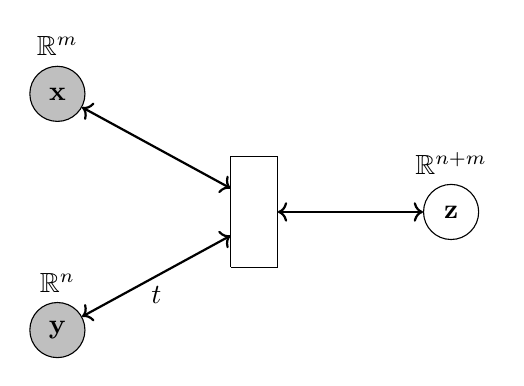
\begin{tikzpicture}
    \node[circle, draw=black, fill=lightgray, minimum size=0.7cm, label={$\mathbb{R}^{n}$}] (y) at (0, 0) {$\mathbf{y}$};
    \node[circle, draw=black, fill=lightgray, minimum size=0.7cm, label={$\mathbb{R}^{m}$} ] (x) at (0, 3) {$\mathbf{x}$};
    \node[circle, draw=black, fill=white, minimum size=0.7cm, label={$\mathbb{R}^{n + m}$}] (z) at (5, 1.5) {$\mathbf{z}$};
    
    \draw (2.2, 0.8) -- (2.8, 0.8) -- (2.8, 2.2) -- (2.2, 2.2) -- (2.2, 0.8);
    
    \draw[<->, thick] (x) to (2.2, 1.8);
    \draw[<->, thick] (y) to node[below] {$\mathbbf{t}$} (2.2, 1.2);
    \draw[<->, thick] (2.8, 1.5) to (z);
\end{tikzpicture}
\end{document}